\documentclass[a4paper,french,11pt,openany,oneside]{memoir}

\usepackage[a4paper]{geometry}
\usepackage[utf8]{inputenc}
\usepackage[T1]{fontenc}
\usepackage{babel}
\usepackage{listings,xcolor}
\usepackage{textcomp}
\usepackage{titling}
\usepackage{graphicx}
\usepackage{appendix}
\usepackage{xpatch}
\usepackage{bookmark}
\usepackage{hyperref}

% Annexes
\renewcommand{\appendixtocname}{Annexes}

% Configure subtitle
\newcommand{\subtitle}[1]{
  \posttitle{
    \par\end{center}
    \begin{center}\large#1\end{center}
    \vskip0.5em}
}

% Configure lists
\renewcommand{\FrenchLabelItem}{\textbullet}

% Configure source code
\definecolor{dkgreen}{rgb}{0,.6,0}
\definecolor{dkblue}{rgb}{0,0,.6}
\definecolor{dkyellow}{cmyk}{0,0,.8,.3}

\lstset{
  basicstyle       = \small\ttfamily,
  numbers          = left,
  columns          = fullflexible,
  showstringspaces = false,
  literate=
  {á}{{\'a}}1 {é}{{\'e}}1 {í}{{\'i}}1 {ó}{{\'o}}1 {ú}{{\'u}}1
  {Á}{{\'A}}1 {É}{{\'E}}1 {Í}{{\'I}}1 {Ó}{{\'O}}1 {Ú}{{\'U}}1
  {à}{{\`a}}1 {è}{{\`e}}1 {ì}{{\`i}}1 {ò}{{\`o}}1 {ù}{{\`u}}1
  {À}{{\`A}}1 {È}{{\'E}}1 {Ì}{{\`I}}1 {Ò}{{\`O}}1 {Ù}{{\`U}}1
  {ä}{{\"a}}1 {ë}{{\"e}}1 {ï}{{\"i}}1 {ö}{{\"o}}1 {ü}{{\"u}}1
  {Ä}{{\"A}}1 {Ë}{{\"E}}1 {Ï}{{\"I}}1 {Ö}{{\"O}}1 {Ü}{{\"U}}1
  {â}{{\^a}}1 {ê}{{\^e}}1 {î}{{\^i}}1 {ô}{{\^o}}1 {û}{{\^u}}1
  {Â}{{\^A}}1 {Ê}{{\^E}}1 {Î}{{\^I}}1 {Ô}{{\^O}}1 {Û}{{\^U}}1
  {œ}{{\oe}}1 {Œ}{{\OE}}1 {æ}{{\ae}}1 {Æ}{{\AE}}1 {ß}{{\ss}}1
  {ç}{{\c c}}1 {Ç}{{\c C}}1 {ø}{{\o}}1 {å}{{\r a}}1 {Å}{{\r A}}1
  {€}{{\EUR}}1 {£}{{\pounds}}1
}


% And meta data

\title{Rapport d'activité n°1}
\author{Loïc \bsc{Payol} - DUT Informatique \\ \\
Anthony \bsc{Cor} -- Falcon Training Center \\ Laurent \bsc{Audibert} -- Université Paris 13}
\date{27 février 2015}

\renewcommand{\maketitlehookd}{%
  \begin{center}
    \vfill
    
\includegraphics[scale=0.8]{img/UnivParis13.png}\\
    
\includegraphics[scale=0.8]{img/FlightSafety.png}\\[\bigskipamount]
  \end{center}
  \newpage
}

\newcommand{\mychapter}[2]{
    \setcounter{chapter}{#1}
    \setcounter{section}{0}
    \chapter*{#2}
    \addcontentsline{toc}{chapter}{#2}
}

\begin{document}
\pagenumbering{arabic}

\thispagestyle{plain}
\maketitle
\begin{KeepFromToc}

\tableofcontents
\newpage

\chapter*{Remerciements}
\thispagestyle{plain}

Je remercie Laurent \bsc{Audibert}, mon tuteur et professeur, de m'avoir suivi tout au long de ce semestre.

J'en profite pour remercier toute l'équipe pédagogique de la formation informatique en alternance à l'université de Villetaneuse pour leur accompagnement, tout particulièrement Oriane \bsc{Deselligny} qui m'a permis de trouver mon entreprise d'accueil.

Je remercie également le \bsc{CFA Sup 2000}, mon centre de formation d'apprentis, de nous encadrer et nous permettre cette intégration dans un milieu professionnel, plus particulièrement Bénedicte \bsc{Cardiet} pour ses précieux conseils lors de mes recherches de contrat.
\\

Je tiens tout particulièrement à remercier Anthony \bsc{Cor}, mon maître d'apprentissage, de m'avoir permis de réaliser ce premier semestre au sein de son entreprise.

Enfin, je souhaite remercier tous les collaborateurs de \bsc{FlightSafety International} pour leur très chaleureux accueil au sein de leur entreprise, ainsi que pour leur sympathie et leur professionnalisme, plus particulièrement mes collègues du service informatique, Christophe \bsc{Enilorac}, Nicolas \bsc{Souques} et Florian \bsc{Besnard}, alternant en DUT Informatique, S3, à Villetaneuse.

\end{KeepFromToc}

\chapter*{Introduction}
\addcontentsline{toc}{chapter}{Introduction}

J'ai pu intégrer la formation pour le DUT Informatique en alternance à Villetaneuse lors de la rentrée de septembre 2014. Dès l'acceptation de mon dossier d'inscription à l'université, il m'a fallu trouver une entreprise d'accueil. Grâce à l'aide de l'équipe pédagogique de mon université, j'ai pu entrer en contact avec FlightSafety International, et intégrer leur structure. Cela fait maintenant un semestre que je travaille au sein de leur service informatique, et ce rapport a pour but de présenter mes activités tout au long de cette période.

\part{Présentation de l'entreprise d'accueil}

\chapter{Généralités}

\section{Historique}

FlightSafety International est une compagnie américaine d'entraînement aéronautique crée en 1951. Elle formait alors des pilotes de la marine de l'air américaine avec, au départ, un seul modèle de simulateur de vol qu'elle louait. Au fil des années, elle fait l'acquisition de plus en plus de simulateurs, s'étend dans plusieurs états d'Amérique, puis dans plusieurs pays, dont la France. Elle est aujourd'hui une filiale du groupe Berkshire-Hathaway et a plus de 4400 employés dans tous ses centres, qui sont au nombre de 37, sur les 5 continents du monde. Enfin, l'organisation a 135 formations professionnelles approuvées, 300 modèles de simulateurs différents, 1800 instructeurs, plus de 3500 cours pour tout professionnel de l'aéronautique, et plus d'un million d'heures d'entraînement.


\section{Le centre FlightSafety International -- Falcon Training Center du Bourget}

\subsection{Gérance}

A l'aéroport du Bourget, le centre FlightSafety International a 10 simulateurs de vols, dont 6 simulteurs de \emph{Falcon}, séries d'avion privés de Dassault, faisant de ce centre un \emph{Falcon Training Center}. Ainsi, le centre apppartient quasiment à moitié à Dassault, certains employé sont rattachés à FlightSafety, d'autres à Falcon Training Center, ce qui est personellement mon cas.

\subsection{Missions}

Pareillement au permis de conduire classique, il faut des licences pour piloter un avion : une licence d'aviation générale, puis une ou plusieurs licences spécifiques à un modèle d'avion particulier. Ce sont ces dernières formations que FlightSafety International assure et propose aux pilotes qui viennent se former. Notre entreprise donne également des cours de maintenance (mécaniciens, éléctriciens ...) ainsi que des formations d'hôtes/hôtesses de l'air.

\chapter{Structure de l'entreprise}

\section{Le holding Berkshire-Hathaway}

En 1996, Berkshire-Hathaway, groupe de holding américain, achète FlightSafety International, rejoignant ainsi un groupe de 55 filiales. Berkshire exerce donc sur FlightSafety une autorité relativement importante, bien que cela ne se perçoive pas ou peu au niveau du salarié. On peut tout de même noter que Berkshire-Hathaway a récemment mis en place chez toutes ses sociétés filles une politique anti-corruption, suite à des polémiques chez l'une des filiales du groupe, exemple de pouvoir au niveau salarial que peut avoir une société de holding.

\section{Le centre FlightSafety du Bourget}

Cette section est résumée par un organigramme, en annexe \ref{figure-fsi-ftc}, page \pageref{figure-fsi-ftc}

\subsection{Formation des pilotes}

Pour assurer la formation des clients, l'entreprise répartit les tâches de la manière suivante : \\

\begin{itemize}
	\item Le \textbf{Head of Training} (HoT) supervise toutes les formations dispensées dans le centre.
	\begin{itemize}
		\item Le \textbf{Director of Training} (DoT) est responsable de l'intégrité des cours.
		\begin{itemize}
			\item Le \textbf{Director of Maintenance Training} (DoMT) s'occupe des cours de maintenance.
		\end{itemize}

		\item Le \textbf{Director of Standards} (DoS) prend en charge la standardisation des licences pilotes.
		\begin{itemize}
			\item Le \textbf{Director of Maintenance Standards} (DoMS) a le même travail, mais pour les cours relatifs aux certifications de maintenance.
		\end{itemize}

		\item Les \textbf{Program Managers} (PM) sont responsables des instructeurs de l'avion pour lesquels ils sont en charge. Dans l'annexe~\ref{figure-fsi-ftc}, ils sont identifiés par le nom de l'avion qui leur est attribué.
	\end{itemize}
\end{itemize}

\subsection{Services internes de l'entreprise}

Pour faire vivre l'entreprise, différents services ont été crées : \\

\begin{itemize}
	\item Le service \textbf{Simulator Maintenance}, qui s'occupe de la maintenance des simulateurs.
	\item Le service \textbf{Customer Support}, qui joue le rôle d'interface avec l'extérieur.
	\item Le service \textbf{Facilities}, qui regroupe le service informatique et le service bâtiment, nous y reviendrons.
	\item Le service \textbf{Finance}, qui est en charge des finances.
	\item Le service \textbf{Sales}, qui recherche des éventuels clients.
	\item Le service \textbf{Logistics}, qui s'occupe de la logistique dans le bâtiment.
	\item Le service \textbf{Human Resources}, qui est responsable des ressources humaines.
\end{itemize}


\section{Le service \emph{Facilities}}

Cette section est résumée par un organigramme, en annexe \ref{figure-facilities}, page \pageref{figure-facilities}. \\

Comme dit précédemment, le services \emph{Facilities} regroupe en réalité deux services distincts : le service informatique, et le service bâtiment. \\

\begin{itemize}
	\item Le \textbf{Facilities Manager} supervise les activités des services généraux.
	\begin{itemize}
		\item Le \textbf{Network Manager}, Anthony \bsc{Cor}, dirige le service informatique.
		\begin{itemize}
			\item Les \textbf{Network Administrators} s'occupe de l'administration du parc informatique.
			\item Les \textbf{IT Technicians} sont chargés de la maintenance du matériel informatique.
		\end{itemize}
		
		\item Le \textbf{Building Manager} est responsable du service \emph{Building}
		\begin{itemize}
			\item Les \textbf{Electrician Technicians} prennent en charge la maintenance des bâtiments de l'entreprise.
		\end{itemize}
	\end{itemize}
\end{itemize}

Je suis donc un technicien dans le service informatique, et comme mon collègue alternant, nous avons comme mission supplémentaire le développement d'applications pour l'entreprise.


\part{Mes missions}

\chapter{Gestion de l'accès aux simulateurs}

Bien que la seule vocation du service informatique est  de réaliser des missions de maintenance (dépannage, installation de salles ...), le service qualité, lors de mon arrivée, m'a proposé une mission de développement. Ce service est en charge de s'assurer de la bonne exécution de chacune des tâches réalisées par l'ensemble des services, dans un souci d'harmonisation entre les différents centres FlightSafety International à travers le monde. Il était donc question de concevoir une base de données ainsi qu'une interface pour y accéder, dans le but de répertorier et d'avoir un suivi des pilotes venant à FlightSafety.

\section{Problématique}

\subsection{Fonctionnement actuel}

Les locaux de l'entreprise sont ouverts 24h/24 afin de permettre aux clients d'utiliser les simulateurs qu'ils ont préalablement réservés, et ce à n'importe quelle heure. Ces pilotes sont soit formés par FlightSafety, soit viennent au nom d'une compagnie aérienne et sont déjà formés. Pour ce dernier cas de figure, on appelle cette location de la \og Dry Lease \fg. Dans le cadre de cette forme de location, la compagnie du pilote loue un simulateur donné pour une durée déterminée, et s'assure de fournir à FlightSafety les documents justificatifs attestant du fait qu'ils soient formés pour le simulateur donné. Le pilote se rend alors au centre et utilise le simulateur. 

\subsection{Problèmes de traçabilité}

A l'heure de mon arrivée à FlightSafety, aucun système de traçabilité des pilotes n'existait. Par exemple, si un objet était perdu dans un simulateur, il était impossible de savoir qui aurait bien pu l'oublier, problèmes auxquels nous faisons régulièrement face. Au delà de ce simple problème d'ordre pratique, il est surtout question d'une faille de sécurité au sein du bâtiment, car une personne peut entrer et circuler librement dans le hangar des simulateurs, sans que personne ne lui demande compte car aucun contrôle d'accès rigoureux n'est effectué à l'entrée en ce qui concerne la \emph{Dry Lease}. L'idée était donc de proposer un système de badges attribué à chacun de ces pilotes, permettant ainsi de rapidement pouvoir identifier une personne et savoir dans quels simulateur elle est autorisée à aller.

\subsection{Tentatives passées}

Le projet n'est pas nouveau et cette tâche a déjà été confiée à d'anciens stagiaires en informatique, cependant la base de données crée était trop redondante, pas normalisée, et les interfaces d'accès, codées en PHP, étaient trop peu ergonomiques et le code trop peu modulaire pour pouvoir être réutilisé. Cette fois-ci, il fallait donc repartir de zéro, aussi bien d'un point de vue technique que conceptuel.


\section{Démarrage du projet}

Le deuxième jour de travail en entreprise, mon maître d'apprentissage, moi même, et le responsable qualité nous sommes réunis pour commencer à mettre en place le projet. Il était question de m'expliquer en détail comment fonctionne actuellement l'entreprise, afin que je puisse modéliser la situation dans une base de données relationnelle. Il y eut beaucoup d'incompréhension, car le responsable qualité parlait en termes de besoins et s'interrogeait encore à comment résoudre le problème précédemment décrit, alors que j'attendais de cette réunion de pouvoir déterminer ensemble les différents éléments permettant de concevoir ma base de donnée. J'ai pu néanmoins jeter les bases de mon modèle et comprendre brièvement le fonctionnement de l'entreprise.

\section{Développement}

\subsection{Programmation de la base de données}

Pour cette base de données, je suis parti du principe que mon interface d'accès à celle-ci sera un site web accessible depuis le réseau interne de l'entreprise. La technologie web que je maîtrise le mieux est PHP, plus particulièrement avec le framework \emph{Symfony2}. Bien qu'il aurait été plus logique de développer ce site avec des technologies Microsoft (notamment ASP.NET), je ne connais pas ces langages, et je n'aurai pas pu coder un projet de manière propre et modulaire. J'ai donc opté pour Symfony2. Par défaut, ce framework inclut \emph{Doctrine2}, un ORM \footnote{Object Relationnal Mapper, Mapping Objet-Relationel en français} permettant, à partir de classes PHP, de générer une base de données et toutes les requêtes qui me permettront d'interagir avec. De par sa nature d'ORM, il faut donc définir pour lui des classes et leur caractéristiques, en l'occurrence, décrire ce qu'est un pilote, un simulateur, une formation ... ainsi que les relations entre les différents objets, dans notre cas, un pilote a plusieurs formations, et une formation est donnée pour un simulateur précis, je reviendrai plus tard sur ce point.

\subsection{Interface d'accès}

Pour programmer le site jouant le rôle d'interface avec la base de données, je pensais au départ à une sorte de bureau virtuel donnant accès à plusieurs applications. Ce gestionnaire d'accès serait une des applications, mais on peut imaginer que par la suite l'intranet serait enrichi avec d'autres applications. J'ai abandonné cette idée, car elle nécessitait de gérer deux projets différents : le serveur d'une part, et le client d'une autre part qui serait en l'occurrence une {\em Single Page Application}\footnote{Application web dont toute la logique de mise en forme des données se fait côté client}. L'ampleur d'un tel projet est disproportionné devant la faible portée de ce projet, qui n'a pour but que d'être utilisé par un maximum de 50 personnes. J'ai finalement opté pour une solution plus classique, c'est à dire exécuter toute la logique de traitement de données côté serveur, formater le tout en HTML et envoyer la réponse au client. Un tel projet demande effectivement moins de ressources en temps et en main d'oeuvre, ce qui correspond aux besoins du projet.

\subsection{Versionnage du code}

Pour travailler sur un projet professionnel, il est essentiel de pouvoir avoir une trace de toutes les modifications que j'effectue sur mon projet. J'ai donc utilisé un logiciel de gestion de version, en l'occurrence Git. Développé par les créateurs du noyau Linux, il est reconnu comme le plus complet et le plus efficace à ce jour. Avec un tel système, je peux travailler simultanément sur plusieurs fonctionnalités, ainsi que sur plusieurs états du site (développement, production ...). Ces différentes versions sont appelées \og branches \fg par Git, et représente un état particulier du projet. Il existe plusieurs modèles en ce qui concerne la gestion de ces branches. J'ai choisi un modèle connu sous le nom de \og Git Flow \fg.

\begin{center}
\begin{figure}[ht]
\centering
     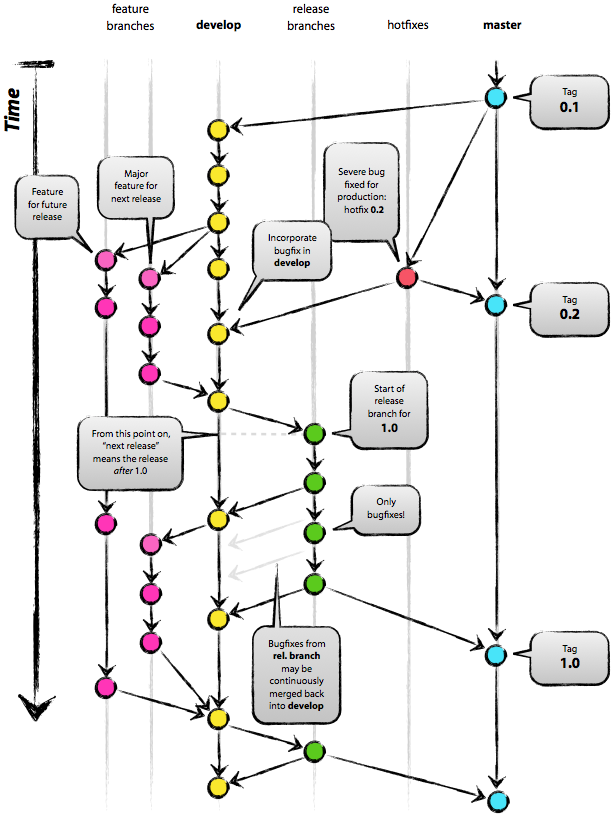
\includegraphics[width=285px]{img/gitflow}
      \caption{Illustration du modèle \og Git Flow \fg }
\end{figure}
\end{center}

Ce modèle permet :

\begin{itemize}
	\item de conserver un état stable du projet, sur la branche \textbf{master}
	\item de corriger rapidement des failles du projet stable, sur la branche \textbf{hotfix}
	\item de développer de nouvelles fonctionnalités sur les branches \textbf{features}
	\item de rassembler ces fonctionnalités fraîchement crées sur la branche \textbf{develop}
	\item de préparer un déploiement de site sur les branches \textbf{release}
\end{itemize}



Il s'agit là d'un modèle robuste pour gérer un projet informatique complexe, et pour collaborer avec plusieurs personnes. Bien que je sois pour l'instant le seul développeur, ce modèle reste néanmoins le meilleur moyen de travailler sur de nouvelles fonctionnalités d'un site tout en conservant l'état stable du site, celui qui est en production.


\section{Problèmes rencontrés}

\subsection{Déploiement du site}

Lors de mon arrivée à l'entreprise, j'ai configuré une machine tournant sous Linux pour pouvoir développer dans un environnement relativement moderne. Seulement, pour déployer le site en production, je comptais sur l'un des deux serveurs auxquels nous avons physiquement accès : le premier est le serveur gérant les imprimantes, le second était utilisé pour un service de support informatique qui a été remplacé par un autre qui n'est plus hébergé en local. Ces deux serveurs tournent sur Windows Server 2003, et porter le projet sur un serveur Windows posa de multiples problèmes.
Pour déployer du code PHP sur un serveur IIS\footnote{Internet Information Services : serveur web de Microsoft}, il faut installer et configurer PHP pour IIS. Cependant, les versions de PHP proposées par Microsoft compatibles avec mon projet ne le sont pas avec les serveurs. Il a donc fallu configurer mon propre serveur web avec Apache, qui lui même entrait en conflit avec IIS. Enfin, il fallut installer certaines extensions PHP pour optimiser les performances de mon application, extensions qui n'étaient pas compilées pour ma plateforme cible. Pour faire court, j'ai utilisé des technologies plus appropriées à un environnement Linux qu'à un environnement Windows, ce qui fut la racine de tous les problèmes que j'ai pu rencontrer dans cette phase de déploiement.

\subsection{Conception des requêtes}

Précédemment, je disais à propos des relations entre les différentes entités de ma base de donées qu'\og un pilote a plusieurs formations, et une formation est donnée pour un simulateur précis \fg. Cette idée n'était pas claire pour moi au début de la réalisation du projet, ainsi j'avais mal modélisé mon pilote, et avait relié directement un pilote à des simulateurs. Plus tard, il a fallu que je puisse répondre à cette question : \og Quels sont les pilotes dont au moins une formation est expirée, et pour quel simulateur n'a-t-il plus accès ? \fg. Je me suis finalement rendu compte au bout d'un mois de mon erreur de modélisation, que j'ai finalement pu résoudre en associant les simulateurs non pas aux pilotes, mais aux formations des pilotes. J'ai ensuite pu avoir une meilleure compréhension du problème, mais il me bloqua dans l'avancement du projet, car l'utilité même de ce dernier réside en cette requête, je devais donc m'assurer de son exactitude. Étant donné que je suis le seul développeur dans l'établissement, je n'ai pu demander de l'aide à personne au sein de l'entreprise, et j'ai fini par demander de l'aide sur des forums d'entraide spécialisés, en l'occurrence \emph{Stackoverflow}\footnote{Voir sujet : http://stackoverflow.com/questions/28225992}, site reconnu pour sa communauté de développeurs chevronnés.



\chapter{Missions de maintenance}

\section{Service d'assistance}

Pour répondre aux demandes des employés, un système de gestions de tickets a été mis en place par FlightSafety, le \emph{HelpDesk}. Lorsqu'un employé a un problème ou une demande particulière, il rédige un ticket via une interface en ligne, puis le service informatique reçoit une notification par mail de l'arrivage d'un ticket. L'un des membres du service informatique peut prendre alors en charge la demande, toujours via l'interface en ligne du HelpDesk.

\section{Maintenance du parc informatique}

Étant en charge du parc informatique, plusieurs missions de maintenance du parc informatique m'ont été confiées.

\subsection{Installations}

Pour installer un nouvel ordinateur, nous devons suivre une procédure précise. Ces procédures font partie d'une base de données de connaissance générale, commune à tous les centres FlightSafety, ceci dans un souci d'harmonisation entre les centres.

\subsection{Dépannage}

Aucune procédure particulière de dépannage existe, car tous les problèmes sont différents. Ces missions de dépannage sont très variées : remplacement de cartouche d'imprimante, assistance à l'utilisation d'un logiciel, mise à jour de logiciels ... Certaines procédures, de mise à jour notamment, existent pour s'assurer d'une compatibilité avec nos infrastructures.

\appendix

\chapter{Diagramme d'organisation}

\begin{center}
\begin{figure}[ht]
\centering
     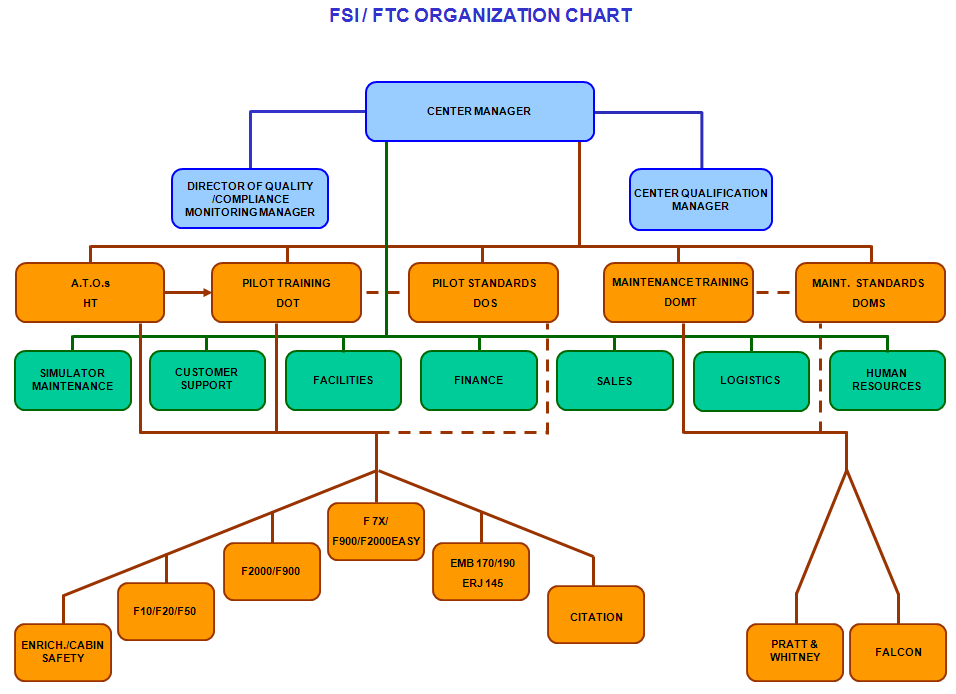
\includegraphics[width=1.0\textwidth]{img/FSIFTC}
      \caption{Diagramme d'organisation du centre FlightSafety du Bourget}
      \label{figure-fsi-ftc}
\end{figure}
\end{center}

\begin{center}
\begin{figure}[ht]
\centering
     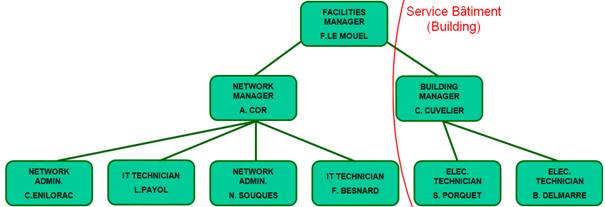
\includegraphics[width=1.0\textwidth]{img/Facilities}
      \caption{Diagramme d'organisation du service \emph{Facilities}}
      \label{figure-facilities}
\end{figure}
\end{center}


\chapter{Définition d'une base de données : l'entité \emph{Pilote}}
\label{entite-pilote}

De par sa qualité d'ORM, Doctrine2, à partir de classes comme celles-ci, peut générer toute une base de données. Ici, ma classe Pilote a des attributs, sur lesquels j'applique des annotations, permettant à Doctrine2 de savoir comment convertir cette classe en table de base de données. La base de données en question peut être représenté par le modèle entités-associations à la figure \ref{entites-associations}, page \pageref{entites-associations}.

Dans le code qui suit, par souci de simplicité, j'ai enlevé toutes les annotations qui ne sont pas utilisées par Doctrine2, car il existe aussi d'autres annotations utilisées par d'autres framework. Aussi, j'ai volontairement éclipsé les méthodes de la classe, car elles n'apportent pas d'intérêt à la compréhension de l'entité.

\begin{lstlisting}[language=php,escapechar=\%]
<?php

namespace FSI\BadgesBundle\Entity;

use Doctrine\ORM\Mapping as ORM;
use Symfony\Bridge\Doctrine\Validator\Constraints\UniqueEntity;

/**
 * Classe représentant un pilote.
 *
 * @ORM\Table()
 * @ORM\Entity(repositoryClass="FSI\BadgesBundle\Entity\PilotRepository")
 * @ORM\HasLifecycleCallbacks
 * 
 * @UniqueEntity("email")
 */
class Pilot
{%\newpage%
    /**
     * @var integer
     *
     * @ORM\Column(name="id", type="integer")
     * @ORM\Id
     * @ORM\GeneratedValue(strategy="AUTO")
     */
    private $id;

    /**
     * @var string
     *
     * @ORM\Column(name="first_name", type="string", length=255, nullable=false)
     */
    private $firstName;

    /**
     * @var string
     *
     * @ORM\Column(name="last_name", type="string", length=255, nullable=false)
     */
    private $lastName;

    /**
     * @var string
     *
     * @ORM\Column(name="photo", type="string", length=256, nullable=false)
     */
    private $photo;

    /**
     * @var \DateTime
     * 
     * @ORM\Column(name="updated", type="datetime", nullable=true)
     */
    private $updated;

    /**
     * @var string
     *
     * @ORM\Column(name="tel", type="string", length=255, nullable=true, unique=true)
     */
    private $tel;%\newpage%
    /**
     * @var string
     *
     * @ORM\Column(name="email", type="string", length=255, nullable=true, unique=true)
     */
    private $email;

    /**
     * @ORM\ManyToMany(targetEntity="Company", inversedBy="pilots")
     * @ORM\JoinTable(name="pilots_companies")
     */
    private $companies;

    /**
     * @ORM\OneToMany(targetEntity="Formation", mappedBy="pilot", cascade="all")
     */
    private $formations;

    /**
     * @ORM\OneToMany(targetEntity="Evaluation", mappedBy="pilot", cascade="all")
     */
    private $evaluations;

    /**
     * @ORM\OneToMany(targetEntity="Remark", mappedBy="pilot", cascade="all")
     */
    private $remarks;
}
\end{lstlisting}

\begin{center}
\begin{figure}[ht]
\centering
    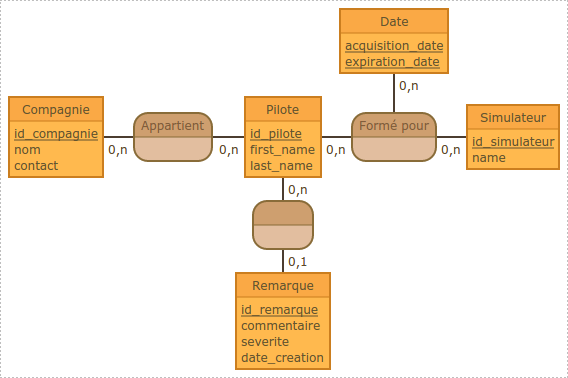
\includegraphics[width=1.0\textwidth]{img/BDD}
    \caption{Modèle entités-associations du gestionnaire de badges}
    \label{entites-associations}
\end{figure}
\end{center}

\chapter{Quelques requêtes avec Doctrine2}
\label{dql-outdated-pilots}

Symfony2 est un framework MVC\footnote{Modèle - Vue - Contrôleur : modèle architectural pour systèmes interactifs}, ce qui signifie que toutes les interactions avec la base de données sont séparés du reste du code. Le code relatif à la base de données, les modèles, sont appelés Repositories. Chaque méthode d'un repository retourne le résultat d'une requête, ces requêtes étant construites avec l'une des plusieurs méthodes proposées par Doctrine, mais celle que j'utilise ici est la DQL\footnote{Doctrine Query Language}, une abstraction du SQL, qui permet d'utiliser un même code sur tous les SGBD\footnote{Système de Gestion de Base de Données} supportés. Le langage est très ressemblant à SQL, il y a quelques subtiles différences qui seront signalées en commentaire du code.
\\

\begin{lstlisting}[language=php,escapechar=\%]
<?php
 
namespace FSI\BadgesBundle\Entity;
 
use Doctrine\ORM\EntityRepository;
use Doctrine\ORM\Query\Expr;
use Application\Sonata\UserBundle\Entity\User; %\newpage%
class PilotRepository extends EntityRepository
{
    public function queryOneWithJoins($id)
    {
        $qb = $this->createQueryBuilder('p')
            ->leftJoin('p.simulators', 's')->addSelect('s')
            ->leftJoin('p.remarks', 'r')->addSelect('r')
            ->leftJoin('p.companies', 'c')->addSelect('c')
            ->leftJoin('p.formations', 'f')->addSelect('f')
            ->leftJoin('p.evaluations', 'e')->addSelect('e')
 
            ->where('p.id = :id')
            ->setParameter('id', $id)
        ;
 
        return $qb;
    }
 
    public function findOneWithJoins($id)
    {
        return
        $this->queryOneWithJoins($id)
             ->getQuery()
             ->getSingleResult()
        ;       
    } 
    
    // ...
    %\newpage%
    public function queryOutdatedPilotsByManager(User $user, \DateTime $threshold = null)
    {
        $em = $this->getEntityManager();
 
        if($threshold == null)
            $threshold = new \DateTime('now');

        $dql = '
            SELECT p1, f1, s1
            FROM FSIBadgesBundle:Pilot p1 '
            /* Au lieu d'utiliser des noms de table
            on utilise les noms des entités */ .'
                INNER JOIN p1.formations f1
                INNER JOIN f1.simulator s1
                INNER JOIN s1.managers m1
            
            WHERE p1.active = TRUE
            AND m1.id = :usrid
            
            AND NOT EXISTS (
                SELECT f2.acquisitionDate
                FROM FSIBadgesBundle:Formation f2
                WHERE f2.acquisitionDate <= :threshold
                  AND f2.expirationDate >= :threshold
                  AND f2.pilot = f1.pilot
                  AND f2.simulator = f1.simulator
            )
        ';
 
        if($threshold != new \DateTime('now'))
        {
            $dql .= '
                AND f1.acquisitionDate <= :now
                AND f1.expirationDate >= :now
                AND f1.expirationDate <= :threshold
            ';
        }
 
        $dql .= '  
            GROUP BY p1, s1
        ';
 
        $query = $em->createQuery($dql);
        $query
           ->setParameter('usrid', $user->getId())
           ->setParameter('threshold', $threshold) //  $threshold est bien un 
           // objet DateTime, pas besoin de convertir, Doctrine s'en occupera
        ;
 
        if($threshold != new \DateTime('now'))
        {
            $query
               ->setParameter('now', new \DateTime('now'))
            ;
        }

 
        return $query;

    }

    public function findOutdatedPilotsByManager(User $user, \DateTime $threshold = null)
    {
        return
        $this->queryOutdatedPilotsByManager($user, $threshold)
             ->getResult()
        ;

    }
 

    public function queryUntrainedPilotsByManager(User $user,\DateTime $threshold = null)
    {
        $qb = $this->createQueryBuilder('p');
        $qb->leftJoin('p.simulators', 's')->addSelect('s')
           ->leftJoin('p.companies', 'c')->addSelect('c')
           ->leftJoin('p.formations', 'f')
           ->leftJoin('s.managers', 'm')
           ->where('p.active = TRUE')
           ->andWhere('f.id IS NULL')
           ->andWhere('m.id = :usrid')
           ->setParameter('usrid', $user->getId());
        return $qb->getQuery();
    }
    
    // ...
    %\newpage%
    public function findUntrainedPilotsByManager(User $user, \DateTime $threshold = null)
    {
        return $this->queryUntrainedPilotsByManager($user, $threshold)->getResult();
    }
}
\end{lstlisting}

\backmatter

\bookmarksetup{startatroot}% this is it
\chapter{Conclusion}

Au terme de ce semestre, j'ai pu acquérir une première expérience professionnelle au sein d'une entreprise. J'ai ainsi pu, au fil des missions qui m'ont été confiées, apprendre à travailler au sein d'une équipe, et plus largement au sein d'une organisation. J'ai pu endosser pleinement un rôle de meneur de projet, car pour mon projet de développement, il était question de livrer mon produit à un client, ici l'entreprise. J'ai ainsi acquis une grande liberté vis-à-vis de mes choix lors de la réalisation de ce site, bien qu'ils ne soient pas toujours les meilleurs. Néanmoins, le projet arrive bientôt en phase de déploiement final, après la rédaction d'une documentation complète. \\

Malgré une intégration relativement longue (vocabulaire propre à l'aéronautique à assimiler, procédures parfois complexes et peu détaillées ...), j'ai réussi à acquérir au fil des semaines une certaine autonomie, et à mieux appréhender les missions de maintenance. Étant donné que la plupart du temps que j'ai passé en entreprise était consacré au développement de mon site web, j'ai encore beaucoup à apprendre, et j'espère pouvoir enrichir mes connaissances dans le domaine tout au long de mon apprentissage. \\

Je suis donc enchanté d'avoir pu contribuer à l'activité de FlightSafety, et j'espère continuer à apporter toujours plus de dynamisme au sein du centre.
\end{document}
